\section{Simulations}\label{sec:5}

\subsection{Design}\label{sec:5a}

I simulate a fuzzy DID design with nonlinear nuisance functions and a high-dimensional covariate dictionary to stress-test the first-step learners. The DGP satisfies Assumptions~\ref{ass:1}--\ref{ass:5}, Assumption~\ref{ass:4prime}, and the third point of Assumption~\ref{ass:8x}, so both Wald-DID and TC are identified. $\Lambda(\cdot)$ denotes the logistic CDF.

\medskip
\noindent\textit{Covariates and assignment.}
\begin{alignat*}{2}
    & X \sim \mathcal{N}(0,\Sigma), \quad \Sigma_{jk} = 0.5^{|j-k|} \cdot 2.25, \quad p_0 = 20 \\
    & T \sim \text{Bernoulli}(0.5), \quad G \sim \text{Bernoulli}\big(\Lambda(0.6 X_1 + 0.3 X_3)\big)
\end{alignat*}

\noindent\textit{Outcome.}
\begin{alignat*}{2}
    & g_0(X) = \Lambda(X_1) + 0.3 X_3 + 0.3 X_1 X_3 + 0.2 X_2^2 + 0.15 X_4 \\
    & h(X) = 0.4 X_1 + 0.2 X_1^2 + 0.15 X_3 \\
    & Y(0) = 0.3\, G + h(X)\, T + g_0(X) + \varepsilon, \quad \varepsilon \sim \mathcal{N}(0,1) \\
    & Y(1) = Y(0) + \Delta + \zeta, \quad \zeta \sim \mathcal{N}(0, 0.25), \quad \Delta = 1
\end{alignat*}

\noindent\textit{Treatment.}
\begin{alignat*}{2}
    & V = G + 0.4 X_1 + 0.2 X_3 + \nu, \quad \nu \sim \mathcal{N}(0,1) \\
    & D(t) = \mathbbm{1}\{V > v_{gt}\}, \quad v_{11} = 0, \quad v_{10} = v_{01} = v_{00} = 2
\end{alignat*}
The design is constructed to exhibit three features relevant to the estimators. First, the outcome functions $g_0$ and $h$ contain nonlinear terms ($\Lambda(X_1)$, $X_1 X_3$, $X_2^2$) that a linear Lasso cannot represent, even in population; the specification bias that contaminates the plug-in estimators is a direct consequence. Second, the propensity score $\Pr(G=1\mid X) = \Lambda(0.6 X_1 + 0.3 X_3)$ is sparse and logistic-linear, so logit-Lasso is correctly specified and the propensity step is not itself a source of bias. Third, the first-stage compliance $DID_D(X)$ depends on $X$ through the latent index $V$, violating first-stage independence (Assumption~\ref{ass:T2}) so the general, rather than the simplified, trimming rule applies. $G$ and $h(X)$ share $X_1, X_3$, so unconditional parallel trends fails, but conditional on $X$ the outcome trend $h$ does not depend on $G$ and Assumption~\ref{ass:4} holds.

To stress-test regularization, I augment $X$ with 80 noise covariates $X_{21}, \ldots, X_{100}$, each correlated ($\rho = 0.3$) with one of the five signal covariates, giving total dimension $p = 100$. Lasso uses all 100 columns and must select the relevant variables from a dictionary that is mostly noise. Because treatment status $D$ depends on $X$ through $V$, the conditional variance of $Y \mid X$ is not constant, so the homoskedasticity assumption underlying Conjecture~\ref{cor:onesided} is violated and the one-sided trimming rule is an approximation in this DGP.

\paragraph{Estimators.} I compare five estimators. \textbf{Wald} is the Wald-DID ratio~\eqref{eq:Wdid} without covariates. \textbf{Wald$_X$} plugs Lasso-estimated $\hat m^R_{gt}(X)$ into~\eqref{eq:5} on the full sample, with no cross-fitting or FSIF correction. \textbf{TC$_X$} does the same for the TC moment~\eqref{eq:6}. Non-DML estimators trim propensities symmetrically at $[0.10, 0.90]$. \textbf{DML-Wald}~\eqref{eq:13} and \textbf{DML-TC}~\eqref{eq:14} are the proposed estimators, built with $L=5$-fold cross-fitting, the FSIF correction of Proposition~\ref{prop:2}, and the data-driven one-sided trimming rule of Section~\ref{sec:4c}.

\subsection{Simulation results}\label{sec:5c}

Table~\ref{tab:main_sim} reports bias, RMSE, standard-error, and coverage across $M=1{,}000$ replications at sample sizes $n \in \{100, 500, 1{,}000, 2{,}000, 5{,}000\}$. The comparison isolates how each estimator handles the nuisance structure. As more of the nonlinear component is absorbed, bias falls sharply. Because the identification assumptions for both estimands hold throughout the design (Assumptions~\ref{ass:1}--\ref{ass:5} and \ref{ass:4prime}), the comparison between Wald and TC is not about identification but about finite-sample performance under misspecified first steps.

The unconditional Wald estimator remains severely biased. Absolute bias stays at $1.05$ log points at every $n$, and coverage falls from $0.88$ at $n=100$ to zero at $n=5{,}000$ as the confidence interval contracts around the wrong value. A linear Lasso plug-in absorbs part of the nuisance structure and reduces bias, but not enough. Wald$_X$ lowers bias to $0.56$ at $n=5{,}000$ and reduces RMSE by $44\%$ relative to Wald; TC$_X$ cuts the remaining bias roughly in half. The nonlinear terms $\Lambda(X_1)$, $X_1X_3$, and $X_2^2$ remain misspecified, and inference remains poorly calibrated. TC$_X$ coverage never rises above $0.78$. The FSIF correction removes most of this remaining error. At $n=5{,}000$, DML-Wald reduces bias from $0.56$ under Wald$_X$ to $0.11$, lowers RMSE by a further $40\%$, and delivers coverage between $0.89$ and $0.90$ with $\overline{SE}/SD$ calibration between $0.90$ and $0.94$ for $n \geq 1{,}000$. DML-TC is the lowest-bias estimator at every sample size. Its bias advantage over DML-Wald is large at small and moderate $n$ and narrows as both estimators converge. Under the misspecified linear Lasso used here, Proposition~\ref{prop:3} guarantees only local robustness as $\hat\gamma \to \gamma_0$, but in finite samples the FSIF correction still absorbs most of the specification bias.

The comparison between DML-Wald and DML-TC is a standard bias-variance trade-off. DML-TC dominates on bias at every $n$ and on coverage once $n \geq 2{,}000$, reaching $0.95$ coverage at $n=5{,}000$ against $0.90$ for DML-Wald. DML-Wald dominates on RMSE from $n=1{,}000$ onward, with gains of $28\%$, $24\%$, and $6\%$ at $n=1{,}000$, $2{,}000$, and $5{,}000$. DML-TC is the right choice when bias control and large-sample inference are the main concern; DML-Wald is the right choice when RMSE matters most at moderate sample sizes.

Two other results are worth to mention. First, the data-driven trimming rule of Section~\ref{sec:4c} closely tracks the RMSE-minimizing threshold and materially improves DML-Wald at small $n$. Its RMSE falls from $7.30$ to $2.33$ at $n=100$, from $1.02$ to $0.88$ at $n=500$, from $0.76$ to $0.66$ at $n=1{,}000$, and from $0.53$ to $0.51$ at $n=2{,}000$. The gain comes with some loss in coverage at larger $n$. DML-TC is largely insensitive to the trimming rule because its score does not load directly on the propensity odds ratio $e/(1-e)$. Second, Table~\ref{tab:ml_comparison} shows that these conclusions are not specific to Lasso. Random forest delivers the lowest DML-TC RMSE, about $5\%$ below Lasso at $n=2{,}000$; the neural network improves coverage modestly at a substantial RMSE cost. Across learners, coverage stays between $0.86$ and $0.95$ for $n \geq 500$, which suggests the FSIF correction does not hinge on the particular first-step method.

\begin{figure}[H]
    \centering
    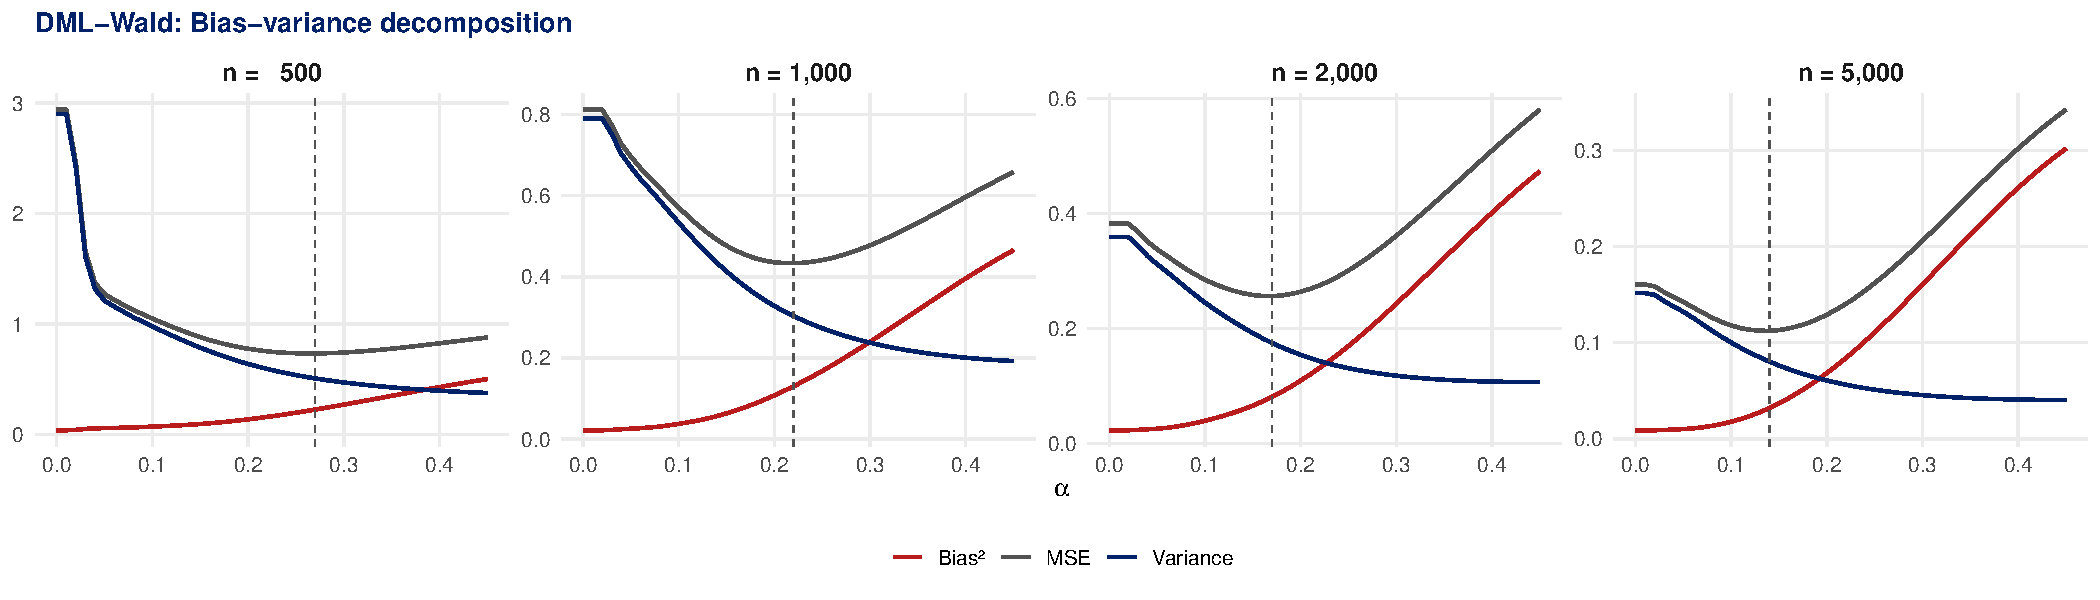
\includegraphics[width=\linewidth]{../output/figures/sim_trimming_wald.pdf}
    \caption[DML-Wald: bias-variance decomposition by trimming threshold]{DML-Wald: bias-variance decomposition as a function of the trimming threshold $\alpha$. Dashed vertical line marks the RMSE-minimizing $\alpha$ at each $n$. The data-driven rule of Section~\ref{sec:4c} selects $\hat\alpha$ near the RMSE-minimizing threshold without knowledge of the true parameter.}\label{fig:trim_wald}
\end{figure}
